\chapter{Biểu diễn và đối đồng điều của $SL_2(\Z)$}
Từ phân tích amalgam cho $SL_2[1/m]$ trong Hệ quả \ref{cor:sl2-amalgam} và dãy khớp dài cho đối đồng điều của tích amalgam trong Mệnh đề \ref{prop:long-seq-amalgam}, ta thấy được ngay bước đầu tiên trong công cuộc tính đối đồng điều của $SL_2[1/m]$ chính là tính đối đồng điều của $SL_2(\Z)$.

\section{Tập sinh của $SL_2(\Z)$}
Trước hết ta nhắc lại định nghĩa
$$
    SL_{2}(\Z) \ =\ \left\{\begin{pmatrix}
        a & b \\
        c & d
    \end{pmatrix} \ \middle\vert\ a,b,c,d\ \in \Z,\ ad-bc=1\right\}
$$
Bằng lập luận đại số thuần thúy, ta có thể mô tả tập sinh cho $SL_2(\Z)$ như sau.

\begin{proposition}
    Đặt
    $$
        S = \begin{pmatrix}
            0 & -1 \\
            1 & 0
        \end{pmatrix} ,\ T=\begin{pmatrix}
            1 & 1 \\
            0 & 1
        \end{pmatrix}.
    $$
    Khi đó $SL_2(\Z) = \langle S, T \rangle$.
\end{proposition}

\startproof Trước hết ta nhận thấy $S$ có cấp $4$ và $T$ có cấp vô hạn, trong đó $S^{2} = -I$ và $T^{n} =\begin{pmatrix}
        1 & n \\
        0 & 1
    \end{pmatrix}$. Xét $\gamma = \begin{pmatrix}
        a & b \\
        c & d
    \end{pmatrix}$, ta có
$$
    S\gamma =\begin{pmatrix}
        -c & -d \\
        a  & b
    \end{pmatrix} \text{ và } T^{n} \gamma =\begin{pmatrix}
        a+cn & b+dn \\
        c    & d
    \end{pmatrix}
$$
Ta sẽ tìm biểu diễn của $\gamma$ thông qua trên $S$ và $T$ dựa trên thuật toán sau:

\begin{enumerate}[(1)]
    \item Nếu $|a| < |c|$ thì thực hiện bước (2) với $\gamma$ thay bằng $S \gamma$.
    \item Nếu $|a| \geq |c|$ và $c \neq 0$. Đặt $n = -q$. Bằng thuật chia Euclid, ta có $a = cq + r$ với $0 \leq r < |c|$. Khi đó $a + cn < r < |c|$, nghĩa là ma trận $T^n \gamma$ lúc này có số hạng vị trí $(1,1)$ bé hơn trị tuyệt đối của số hạng vị trí $(2,1)$. Quay lại bước (2) với $\gamma$ thay bằng $ST^n \gamma$.
    \item Nếu $c = 0$ thì $a = d = \pm 1$, do đó $\gamma = \pm T^{\pm b}$ là biểu diễn cần tìm.
\end{enumerate}

Để ý tại bước (2) do $a + cn$ nhỏ hơn hẳn so với $|c|$ nên thuật toán phải dừng tại hữu hạn bước khi $a + cn = 0$.

\begin{proposition}\label{prop:SR-gen-sl2}
    Đặt $R = TS = \begin{pmatrix}
            1 & -1 \\
            1 & 0
        \end{pmatrix}$. Khi đó $\{S,R\}$ cũng là một tập sinh của $SL_2(\Z)$.
\end{proposition}

\startproof Ta có $T = RS^3 \in \langle S,R \rangle$. Do đó $SL_2(\Z) = \langle S, T \rangle \subset \langle S,R \rangle$.\qed

\begin{remark}
    Để ý rằng $R$ có cấp $6$. Do đó $SL_2(\Z)$ sinh bởi $2$ phần tử có cấp hữu hạn.
\end{remark}

\section{Phân tích amalgam cho $SL_2(\Z)$}
Bằng lý thuyết Bass-Serre, ta có một phân tích amalgam cho $SL_2(\Z)$ dựa trên tác động lên nửa mặt phẳng phức
$$
    \HC = \{ z \in \C\ |\ \im(z) > 0 \}
$$
thông qua phép biến đổi Möbius
$$
    \begin{pmatrix}
        a & b \\
        c & d
    \end{pmatrix} z = \frac{az+b}{cz+d}
$$
với $z \in \HC$. Hơn nữa phân tích này là một cách khác để chứng tỏ $SL_2(\Z)$ sinh bởi $S$ và $T$.

\begin{lemma}\label{lem:fundamental-domain}
    Với $S^1 = \{z \in \C\ |\ |z| = 1\}$ và $\gamma = \begin{pmatrix}
            a & b \\
            c & d
        \end{pmatrix} \in SL_2(\Z)$. Đặt $C = S^1 \cap \HC$. Khi đó ta có
    $$
        \gamma (C) = \left\{z \in \HC:\ \left| z-\frac{ac-bd}{c^{2} -d^{2}}\right| =\frac{1}{|c^{2} -d^{2} |}\right\} ,\  \text{ nếu }  c^{2} \neq d^{2}
    $$
    và
    $$
        \gamma (C) = \left\{z \in \HC:\ \Real( z) =ac-\frac{cd}{2}\right\} ,\ \text{ nếu }  c^{2} =d^{2} =1, cd=\pm 1.
    $$
\end{lemma}

\startproof Nếu $c^2 \neq d^2$, ta có $\gamma(1) = \frac{a+b}{c+d}$ và $\gamma(-1) = \frac{-a+b}{-c+d}$, khi đó tâm và khoảng cách giữa chúng có dạng
$$
    \mu := \frac{\gamma(1) + \gamma(-1)}{2} = \frac{ac-bd}{c^{2} -d^{2}}\quad \text{và}\quad \delta := \left| \frac{\gamma(1) - \gamma(-1)}{2} \right| = \left| \frac{2}{c^2 - d^2} \right|.
$$
Xét
$$
    \gamma(i) = \frac{ai + b}{ci + d} = \frac{b+ia}{d+ic} \cdot \frac{d - ic}{d - ic} = \frac{ac + bd + i}{c^2 + d^2},
$$
suy ra
\begin{align*}
    \left| \gamma(i) - \frac{ac-bd}{c^2-d^2} \right| & = \left| \frac{((ac+bd)(c^2-d^2) - (ac-bd)(c^2+d^2))}{(c^2+d^2)(c^2-d^2)} + \frac{i}{c^2+d^2} \right|              \\
                                                     & = \left| \frac{-2cd+i(c^2-d^2)}{(c^2+d^2)(c^2-d^2)} \right| = \left| \frac{1}{c^2-d^2} \right| = \frac{\delta}{2}.
\end{align*}
Vậy ta có $3$ điểm trên $\gamma (C)$ cùng cách $\mu$ một khoảng $\delta/2$, hơn nữa do biến đổi Möbius biến đường tròn thành đường tròn nên $\gamma (C)$ phải là nửa đường tròn trên $\HC$ tâm $\mu$ bán kính $\delta/2$.

Trong trường hợp $c^2 = d^2$, ta có $cd = \pm 1$, suy ra $1 = ad - bc = c(\pm a - b)$, do đó $d = \pm 1$. Suy ra , $bd = ac - (\pm 1)$ và
\begin{align*}
    \gamma(z) = \frac{az+b}{cz+d} \cdot \frac{c \bar{z} + d}{c\bar{z} + d} & = \frac{ac + adz + bc\bar{z} + bd}{c^2+d^2+cd(z+\bar{z})}           \\
                                                                           & = \frac{ac(1 \pm z) + bd(1 \pm \bar{z})}{2(1 + \Real(z))}           \\
                                                                           & = \frac{2ac(1 \pm \Real(z)) - (\pm 1 + \bar{z})}{2(1 \pm \Real(z))} \\
                                                                           & = ac - \frac{\pm 1}{2} + \frac{\im(z)}{2(1 \pm \Real(z))}i.
\end{align*}
Bằng cách giải phương trình $\frac{\sqrt{1-x^2}}{2(1-x)} = t$ theo $x$, ta tìm được điểm tương ứng trên đường tròn ánh xạ qua đường thẳng có phần thực $ac - \frac{cd}{2}$, do đó $\gamma(C)$ là cả đường thẳng $\left\{z \in \HC:\ \Real( z) =ac-\frac{cd}{2}\right\}$.\qed

\begin{proposition}
    Cung tròn $Y = \{z = e^{i \theta}\ |\ \frac{\pi}{3} \leq \theta \leq \frac{\pi}{2} \} \subset C$ và hai điểm đầu mút $P = e^{\frac{i\pi}{2}} =  i, Q = e^{\frac{i\pi}{3}}$ được minh họa như sau

    \begin{figure}[H]
        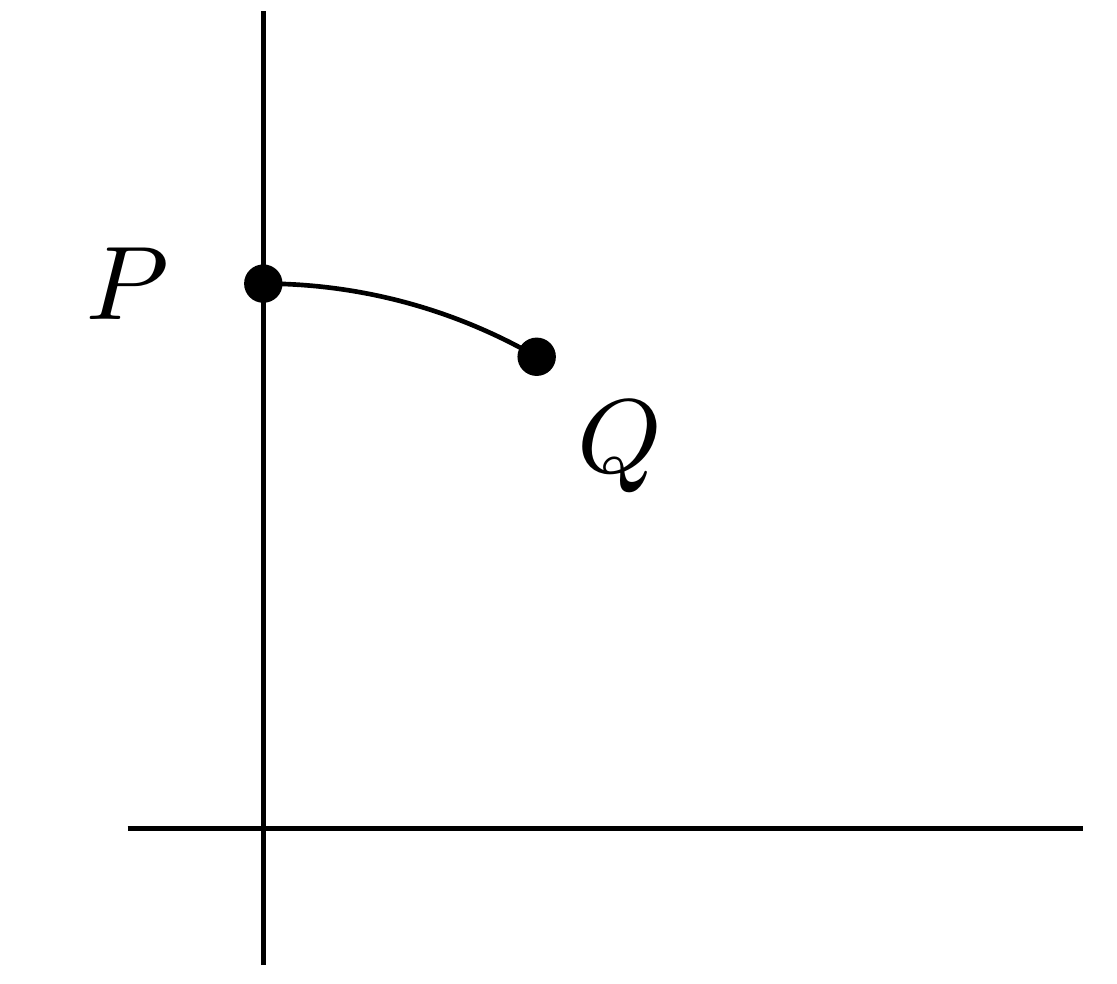
\includegraphics[width=5cm]{assets/circle-segment.png}
        \centering
    \end{figure}
    có nhóm con ổn định đẳng cấu lần lượt với $\Z/2, \Z/4$ và $\Z/6$.
\end{proposition}

\startproof
Do
$$
    \begin{aligned}
        \frac{ai+b}{ci+d} =i & \ \Leftrightarrow\ b+ia=-c+id             \\
                             & \ \Leftrightarrow\  b=-c\ \text{ và } a=d
    \end{aligned}
$$
và $ad - bc = 1$ nên $a^2 + b^2 = 1$. Bằng cách xét 2 trường hợp $a = 0$ hay $b = 0$, ta có $4$ ma trận tương ứng nhóm con cyclic cấp $4$ sinh bởi $S =\begin{pmatrix}
        0 & -1 \\
        1 & 0
    \end{pmatrix}$. Vậy $\langle S \rangle$ là nhóm con cố định $P$. Tương tự ta cũng xét
$$
    \begin{aligned}
        \frac{ae^{i\pi /3} +b}{ce^{i\pi /3} +d} =e^{i\pi /3} & \ \Leftrightarrow\ \left(\frac{a}{2} +b\right) +ia\frac{\sqrt{3}}{2} =\left( -\frac{c}{a} +\frac{d}{a}\right) +i\frac{\sqrt{3}}{2}( c+d) \\
                                                             & \ \Leftrightarrow\ a+2b=d-c\text{ và } a=c+d                                                                                             \\
                                                             & \ \Leftrightarrow\ b=-c\text{ và } a( a-c) +c^{2} =1.
    \end{aligned}
$$
Giải phương trình $a^2-ca+(c^2-1)=0$, ta có $c^2 - 4(c^2-1) \geq 0$ và do đó $|c| \leq \frac{2}{\sqrt{3}} \approx 1.154$. Suy ra ta có các khả năng $c = 0,\ c=1$ hay $c=-1$. Mỗi giá trị của $c$ lại cho ra $2$ giá trị $a$ tương ứng. $b$ và $d$ thì phụ thuộc vào $c$ và $a$. Từ đó ta có $6$ ma trận tương ứng và chúng là các phần tử của nhóm con cấp $6$ sinh bởi $R = \begin{pmatrix}
        1 & -1 \\
        1 & 0
    \end{pmatrix}$. Suy ra $\langle R \rangle$ là nhóm con cố định $Q$.

Nhóm con ổn định $Y$ phải nằm trong phần giao $\langle S \rangle \cap \langle R \rangle$ và do đó phải bằng $\{I,-I\}$ vì $I$ và $-I$ đều là các tác động tầm thường.\qed

\begin{theorem}
    $X = SL_2(\Z) \cdot Y$ là cây và $Y$ là miền cơ bản dưới tác động của $SL_2(\Z)$ lên $X$. Do đó ta có
    $$
        SL_2(\Z) \cong \Z/4 *_{\Z/2} \Z/6.
    $$
\end{theorem}

\startproof Đầu tiên ta cần chứng tỏ rằng $X$ là nhận dạng của đồ thị, thật vậy ta sẽ chỉ ra rằng dưới tác động của $\gamma$ thì $Y$ chỉ có thể giao với $\gamma (Y)$ tại $\gamma(P)$ hoặc $\gamma(Q)$. Giả sử $\gamma(Y) \cap Y \neq \varnothing$, dựa trên Bổ đề $\ref{lem:fundamental-domain}$, ta chia ra 2 trường hợp.

Nếu $c^2 \neq d^2$, ta có $\frac{1}{|c^2-d^2|} = 1$, vậy $c$ hoặc $d$ bằng $0$ và tâm $\mu = (ac-bd)/(c^2-d^2)$ phải bằng $0$ hoặc $1$. Nếu $\mu = 0$ thì $\gamma$ hoặc $\gamma$ là phép tịnh tiến, nghĩa là phải bằng $\pm I$, hoặc $\gamma = S$ nếu $a = 0$ ($S$ là phép phản xạ $Y$ qua trục $y$  do $S(Y) = -\bar{Y}$). Nếu $\mu = 1$, $d = 0$, $ac = 1$ thì $\gamma = \pm R$ (cố định $Q$).

Nếu $c^2 = d^2 = 1$ thì phần thực phải bằng $1/2$, do đó $a \in \{0,1,-1\}$. Nếu $a = 0$ thì $\gamma = \pm R^2$ (cố định $Q$) và với $a = \pm$ thì phần giao phải bằng rỗng (mâu thuẫn).

$SL_2(\Z)$ được sinh bởi $S$ và $R$ theo Mệnh đề \ref{prop:SR-gen-sl2}, do đó bất kì tác động $\gamma \in SL_2(\Z)$ lên $Y$ đều tương ứng với một chuỗi tác động bởi $S$ và $R$. Ta có $Y$ liên thông với $S(Y)$ và $R(Y)$ và do đó $Y' = S(Y) \cup Y \cup R(Y)$ liên thông, tương tự ta cũng có $Y'' = S(Y') \cup Y' \cup R(Y')$ liên thông. Cứ tiếp tục quá trình trên ta có $X$ là một đồ thị liên thông.

Cuối cùng, ta có $C = S^1 \cap \HC$ chỉ cắt $X$ tại điểm $P=i$ trên trục $y$, suy ra cạnh duy nhất của $X$ cắt trục $y$ là $Y$ và $S(Y)$. Hơn nữa bất kì đường đi nào trong $X$ đều có thể tịnh tiến để cắt trục $y$, do đó nếu $X$ chứa chu trình thì $X$ phải cắt trục $y$ 2 lần, điều này là mâu thuẫn và do đó $X$ là cây. Theo Định lí \ref{thm:bass-serre-fund} ta có điều phải chứng minh. \qed

\begin{figure}[H]
    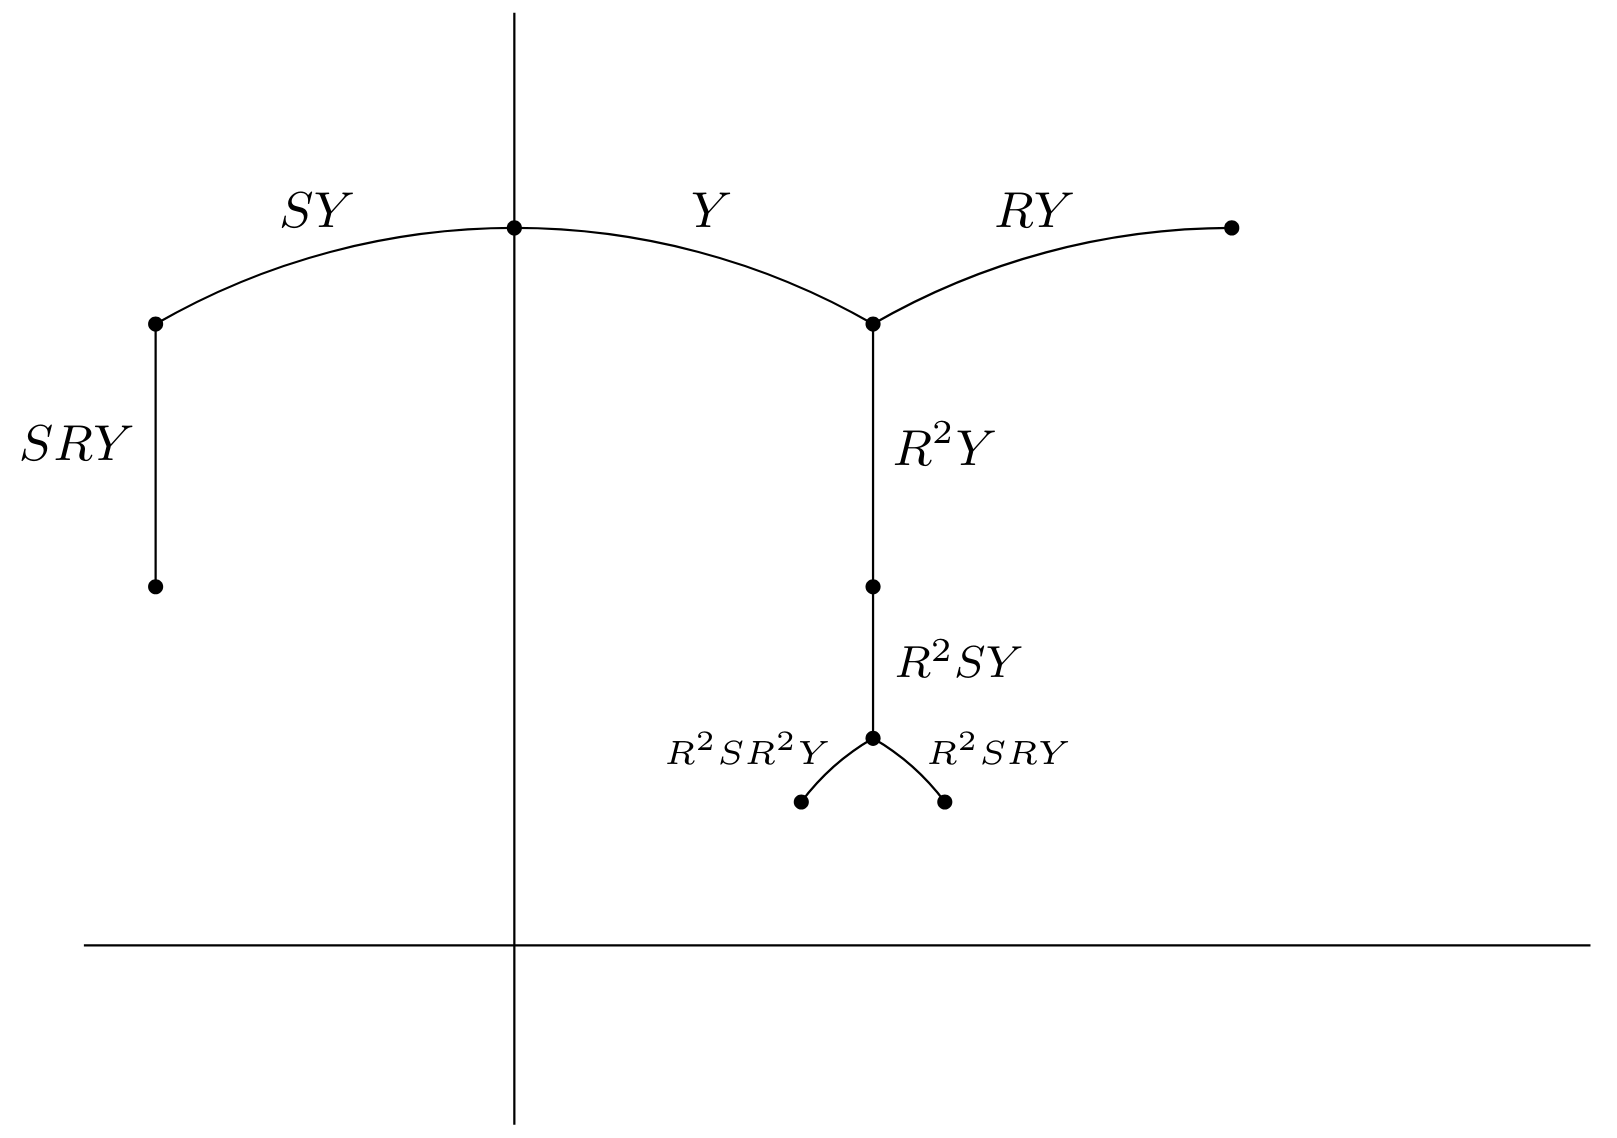
\includegraphics[width=13cm]{assets/sl2z-tree.png}
    \centering
\end{figure}

\begin{corollary}\label{cor:sl2z-presentation}
    Từ phân tích amalgam trên, ta có biểu diễn
    $$
        SL_2(\Z) = \langle R,S\ |\ R^6 = S^4 = 1, R^3 = S^2 \rangle.
    $$
    Ngoài ra với nhóm tuyến tính xạ ảnh đặc biệt $PSL_2(\Z) = SL_2(\Z) / \{\pm I\}$ thì ta cũng có phân tích
    $$
        PSL_2(\Z) \cong \Z/2 * \Z/3.
    $$
    và biểu diễn
    $$
        PSL_2(\Z) = \langle R, S \rangle = \langle R^3 = S^2 = 1 \rangle = \langle S, T\ |\ S^2 = (ST)^3 = 1 \rangle.
    $$
\end{corollary}

\section{Đối đồng điều của $SL_2(\Z)$}
Để tránh nhầm lẫn với phép cộng trong vành nhóm, trong phần này ta kí hiệu $C_n$ viết theo lối nhân cho nhóm cyclic cấp $n$.

\begin{theorem}
    $$
        H^n(SL_2(\Z);\Z) = \begin{cases}
            \Z,      & n = 0               \\
            0,       & n \text{ lẻ}        \\
            \Z / 12, & n > 0 \text{ chẵn}.
        \end{cases}
    $$
\end{theorem}
\vspace{4mm}
\startproof
Gọi $r,s$ và $t$ lần lượt là phần tử sinh của $C_2$, $C_4$ và $C_6$. Ta biết rằng phân tích amalgam của $SL_2(\Z)$ được biểu diễn thông qua các đồng cấu
$$
    \alpha_1: C_2 \rightarrow C_4,\ r \mapsto s^2\ \text{và}\ \alpha_2: C_2 \rightarrow C_6,\ r \mapsto t^3
$$
Sử dụng phép giải cho $C_2$ và $C_4$ mà ta đã đưa ra trong lúc tính đối đồng điều cho nhóm cyclic
$$
    \begin{tikzcd}
        \cdots \arrow[r, "r-1"] & \Z C_2 \arrow[rr, "1+r"] \arrow[d, "f_2"] &  & \Z C_2 \arrow[r, "r-1"] \arrow[d, "f_1"] & \Z C_2 \arrow[r, "\varepsilon_1"] \arrow[d, "f_0"] & \Z \arrow[r] \arrow[d, "\id"] & 0 \\
        \cdots \arrow[r, "s-1"] & \Z C_4 \arrow[rr, "1+s+s^2+s^3"]          &  & \Z C_4 \arrow[r, "s-1"]                  & \Z C_4 \arrow[r, "\varepsilon_2"]                  & \Z \arrow[r]                 & 0
    \end{tikzcd}
$$
ta mong muốn xây dựng ánh xạ dây chuyền $f = \{f_n: \Z C_2 \rightarrow \Z C_4 \}$ giữa hai phép giải, trong đó $f_0$ là mở rộng tuyến tính lên vành nhóm của đồng cấu $\alpha_1: C_2 \rightarrow C_4$. Để ý rằng $f_n$ được xác định duy nhất thông qua $f_n(1)$.

Với $n$ chẵn, giả sử tính giao hoán của biểu đồ trên, ta có
\begin{equation}
    (1+s+s^2+s^3)f_{n+1}(1) = f_n((1+r)\cdot 1) = f_n(1+\alpha_1(r)) = (1+s^2) f_n(1).\label{eq:fn_commute}
\end{equation}
Tác động $s-1$ vào ta được
$$
    0 = (s-1)(1+s+s^2+s^3)f_{n+1}(1) = (s-1)(1+s^2)f_n(1) = (-1+s-s^2+s^3)f_n(1).
$$
Do đó ta có thể chọn $f_n(1) = 1+s$ để thỏa đẳng thức trên. Bây giờ $\ref{eq:fn_commute}$ trở thành thành
$$
    (1+s+s^2+s^3)f_{n+1}(1) = (1+s^2)(1+s) = 1+s+s^2+s^3.
$$
Vậy bằng cách chọn $f_{n+1}(1) = 1$, ta có $f$ là một ánh xạ dây chuyền như mong muốn.

Tiếp theo, ta tác động lần lượt $\Hom_{C_2}(-, \Z)$ và $\Hom_{C_2}(-, \Z)$ vào hai phép giải trên
$$
    \begin{tikzcd}
        \cdots & \Z \arrow[l, "2"']                     & \Z \arrow[l, "0"']                     & \Z \arrow[l, "2"']                     & \Z \arrow[l, "0"']                     \\
        \cdots & \Z \arrow[l, "2"'] \arrow[u, "f_3^*"'] & \Z \arrow[u, "f_2^*"'] \arrow[l, "0"'] & \Z \arrow[l, "4"'] \arrow[u, "f_1^*"'] & \Z \arrow[l, "0"'] \arrow[u, "f_0^*"']
    \end{tikzcd}
$$
Trong đó $f_n^*(1) = 2$ nếu $n$ chẵn và $f_n^*(1) = 1$ nếu $n$ lẻ. Ta biết rằng
$$
    H^n(C_k;\Z) = \begin{cases}
        \Z,  & n = 0               \\
        0,   & n \text{ lẻ}        \\
        C_k, & n > 0 \text{ chẵn}.
    \end{cases}
$$
Từ đó $\{f^*_n\}$ cảm sinh ra đồng cấu $\alpha_1^*: H^n(C_4; \Z) \rightarrow H^n(C_6;\Z)$ là đồng cấu đồng nhất nếu $n = 0$, là đồng cấu tầm thường nếu $n > 0$ lẻ và là đồng cấu biến $s \mapsto r$ nếu $n > 0$ chẵn.

Tương tự ta cũng xây dựng được đồng cấu $\alpha^*_2: H^n(C_6; \Z) \rightarrow H^n(C_2;\Z)$ xác định như trên, với $t \mapsto r$ trong trường hợp $n > 0$ chẵn.

Hai đồng cấu này cảm sinh duy nhất từ $\alpha_1$ và $\alpha_2$, do đó chúng cũng là đồng cấu nối trong dãy khớp dài ở Mệnh đề \ref{prop:long-seq-amalgam}
$$
    \cdots \xrightarrow{} H^{n-1}(C_2) \xrightarrow{\psi} H^n(SL_2(\Z)) \xrightarrow{\varphi} H^n(C_4) \oplus H^n(C_6) \xrightarrow{\alpha_1^* + \alpha_2^*} H^n(C_2) \xrightarrow{} \cdots
$$
trong đó $\alpha_1^* + \alpha_2^*: (a,b) \mapsto a + b$ là toàn ánh với mỗi $n$. Do đó $\psi = 0$ và $\varphi$ là đơn cấu.

Dãy khớp tại $n = 0$ có dạng
$$
    0 \xrightarrow{} H^0(SL_2(\Z)) \xrightarrow{\varphi} \Z \oplus \Z \xrightarrow{} \Z \xrightarrow{} \cdots
$$
Suy ra $H^0(SL_2(\Z)) \cong \im(\varphi) = \ker(\alpha_1^* + \alpha_2^*) = \langle (1,-1) \rangle \cong \Z$. Với $n > 0$ chẵn, ta có
$$
    \cdots \xrightarrow{} H^n(SL_2(\Z)) \xrightarrow{\varphi} C_4 \oplus C_6 \xrightarrow{} C_2 \xrightarrow{} \cdots
$$
Để ý rằng nếu ta viết $C_4$ và $C_6$ theo dạng nhóm cộng modulo thì $\ker(\alpha_1^* + \alpha_2^*)$ là tập các cặp $(a,b)$ sao cho $a$ và $b$ cùng chẵn hoặc cùng lẻ, nghĩa là nhóm có cấp $12$. Hơn nữa nó còn là nhóm cyclic sinh bởi $\langle (1,1) \rangle$. Do đó $H^n(SL_2(\Z)) \cong \im(\varphi) = \ker(\alpha_1^* + \alpha_2^*) \cong C_{12}$. Với $n$ lẻ thì ta có
$$
    \cdots \xrightarrow{} H^{n-1}(C_2) \xrightarrow{} H^n(SL_2(\Z)) \xrightarrow{\varphi} 0 \xrightarrow{} \cdots
$$
do đó $H^n(SL_2(\Z)) = 0$ vì $\varphi$ là đơn cấu. \qed

\begin{corollary}
    Từ Định lí hệ số phổ dụng \ref{cor:universal-coef}, ta cũng tính được đồng điều thứ $n$ của $SL_2(\Z)$ cho bởi
    $$
        H_n(SL_2(\Z);\Z) = \begin{cases}
            \Z,      & n = 0               \\
            \Z / 12, & n \text{ lẻ}        \\
            0,       & n > 0 \text{ chẵn}.
        \end{cases}
    $$
\end{corollary}